\documentclass[conference]{IEEEtran}
\IEEEoverridecommandlockouts
% The preceding line is only needed to identify funding in the first footnote. If that is unneeded, please comment it out.
\usepackage{cite}
\usepackage{amsmath,amssymb,amsfonts}
\usepackage{algorithmic}
\usepackage{graphicx}
\usepackage{textcomp}
\usepackage{xcolor}
\usepackage{hyperref}
\usepackage{float}
\usepackage{subfig}

\def\BibTeX{{\rm B\kern-.05em{\sc i\kern-.025em b}\kern-.08em
    T\kern-.1667em\lower.7ex\hbox{E}\kern-.125emX}}
\begin{document}

\title{Model Driven Approach for Migration Problem in Hybrid App Development\\}

%TODO: Insert names for each team member%
\author{\IEEEauthorblockN{1\textsuperscript{st} Given Name Surname}
\IEEEauthorblockA{\textit{dept. name of organization (of Aff.)} \\
\textit{name of organization (of Aff.)}\\
City, Country \\
email address or ORCID}
\and

\IEEEauthorblockN{Mubtasim Mahmud}
\IEEEauthorblockA{\textit{Faculty of IT} \\
\textit{Monash University}\\
Melbourne, Australia \\
mubtasimmahmud20@gmail.com}
\and

\IEEEauthorblockN{Riordan Dervin Alfredo}
\IEEEauthorblockA{\textit{Faculty of IT} \\
\textit{Monash University}\\
Melbourne, Australia \\
riordan.alfredo@gmail.com}
\and

\IEEEauthorblockN{ Raymond Nguyen }
\IEEEauthorblockA{\textit{Faculty of IT} \\
\textit{Monash University}\\
Melbourne, Australia \\
rbnguyen1357@yahoo.com.au}
}

\maketitle

\begin{abstract}
Software migration is a common problem for developers working in industry or even working on personal projects. It is usually time consuming
and difficult to test if it has been done correctly. Nowadays may web application frameworks have different versions which makes it difficult
to migrate given how frequently they change. One key example is the Ionic Framework which is used to help build desktop as well as mobile applications,
with a simple "write once, deploy anywhere" type of strategy. The Ionic Framework has a manual migration guide that can help developers migrate from 
different versions, however we proposed a model-driven apporach to aid the migration process. By focusing on a model-driven approach, we can develop a model
which is a representation of the system which will generate code for a specific version. Our approach was applied to a case study in order to validate
whether this approach was successful or not. 
\end{abstract}

\section{Introduction}
At some point in the software lifecycle, the current system must be migrated into a new system or version. 
Software migration is the intricate process of moving an application from one environment or version to another. 
Software migration in general, usually consumes lots of resources, time, and effort. 
\\ According to the online article (IBM, 2014) \cite{b1}, it described several common challenges in migrating software applications. In terms of business aspects, these include: determining when to migrate, resistance of users culture and the migration itself not being completed on time. 
For the technical aspects, these include: minimizing disruption of mission critical applications and ensuring that the application functions correctly after migration.
\\ These migration challenges are common for new technologies, especially for web and mobile-based applications as they are constantly changing. Recently, hybrid apps have become popular as an alternative to native mobile applications. Hybrid applications host a web application inside a 
native webview while utilizing bridges that allow access to native app functions such as camera access, geolocation, etc. 
This means that developers are able to carry over their expertise with web technologies to mobile app development without needing to learn native tech stacks. 
\\ A key example of this is the Ionic Framework which is a very popular hybrid application development framework that employs a ‘write once, deploy anywhere’ approach. The latest version of Ionic (version 4) was 
a complete rewrite that makes it incompatible with projects written in Ionic 3, which makes it a suitable candidate for the research project.
\\ There are several differences between Ionic 3 and 4, which makes it worth the port, including compatibility with any front-end framework as opposed to Ionic 3’s tight coupling with Angular. 
There are quite a few issues that can deter development teams from doing a manual port to Ionic 4 which includes breaking changes to the library versions used in both framework versions. Despite there being a guide into how to manually migrate from an Ionic 3 project to an Ionic 4 project, 
there are still a vast number of forums dedicated to help solve the manual migration process. 
\\ One potential solution to solve these problems is to create models to help generate code to support the migration process. 
This might be achieved with a software engineering technique called model-driven development. Model-driven approaches are used mainly in software design to generally 
simplify a complex process of the system into a higher-level abstraction. By abstracting the migration process into a code generation tool, it could possibly speed up the 
migration process with high accuracy and consistency as intended. In addition, it would benefit developers as it is a more efficient way to deal with the migration problems.
\\ Finally, applying a model driven approach would not just be applicable to the Ionic framework, but potentially other web frameworks as well. 
Therefore, model-driven approaches might solve software migration problems towards hybrid app development in regards to technical and business aspects 
that industry is currently facing. Using a model-driven approach as well as focusing on Ionic versions 3 and 4, the research undertaken will determine whether 
the issue of model driven approaches for migration can be applied.
\newline \newline Looking into the problem a bit more, we have devised a main research question below.
\newline \newline \textbf{Can model-driven development provide a valid migration solution?}
\newline \newline Branching away from this primary question, we can ask further questions that target specific concerns about the migration tool we are proposing to create using model-driven development:
\begin{enumerate}
    \item Can it account for major changes like different libraries/versions?
    \newline Looking at the Ionic Framework, there are specific libraries or versions used in a project that may differ from one version to another. 
    These may involve small changes like simply changing the name to match the new version or larger changes such as changing the way the application handles routing to different pages. 
    Our research will involve taking a look at some of these changes.
    \item Is generated code of acceptable quality?
    \newline With the model being used to help convert one Ionic 3 project file to a compatible Ionic 4 version, there can be a chance that the migration may not be perfect. 
    There might be flaws with the output of the conversion which breaks the integrity of the original file. Our research will also observe the quality of the code and take note of any changes.
    \item Can the tool be used for other case studies?
    \newline Our modelling tool will be primarily used for our case study (Meetup For Pets) however every Ionic project is expected to be different. 
    Our research will observe to see if the tool will be applicable not just for our case study, but for other Ionic 3 projects as well. 
\end{enumerate}
The contributions of this work are as follows:
\begin{itemize}
    \item We will introduce a case study Ionic 3 application (MeetUp For Pets) built primarily to test the viability of a proposed model
    \item A metamodel will be built as well as a model which performs code generation to convert from Ionic 3 to Ionic 4
    \item Our findings and evaluations will then be presented on the feasibility of using a model driven approach for migrating using the Ionic Framework as the primary focus
\end{itemize}

\section{Approach}

\subsection{Case Study}
As a proof-of-concept, the application that will be developed for our case study will be called \textbf{Meetups for Pets}. It is a hybrid application written 
in Ionic version 3 to connect pet enthusiasts to promote face-to-face interactions with pets and their owners. The users will have the ability to organise a 
meetups with each pet’s owner. The main purpose of this case study is to test the model-driven migration tool, this can be shown in \ref{fig:meetupIonic}
\begin{figure}%
    \centering
    \subfloat[The home page of Meetup for Pets]{{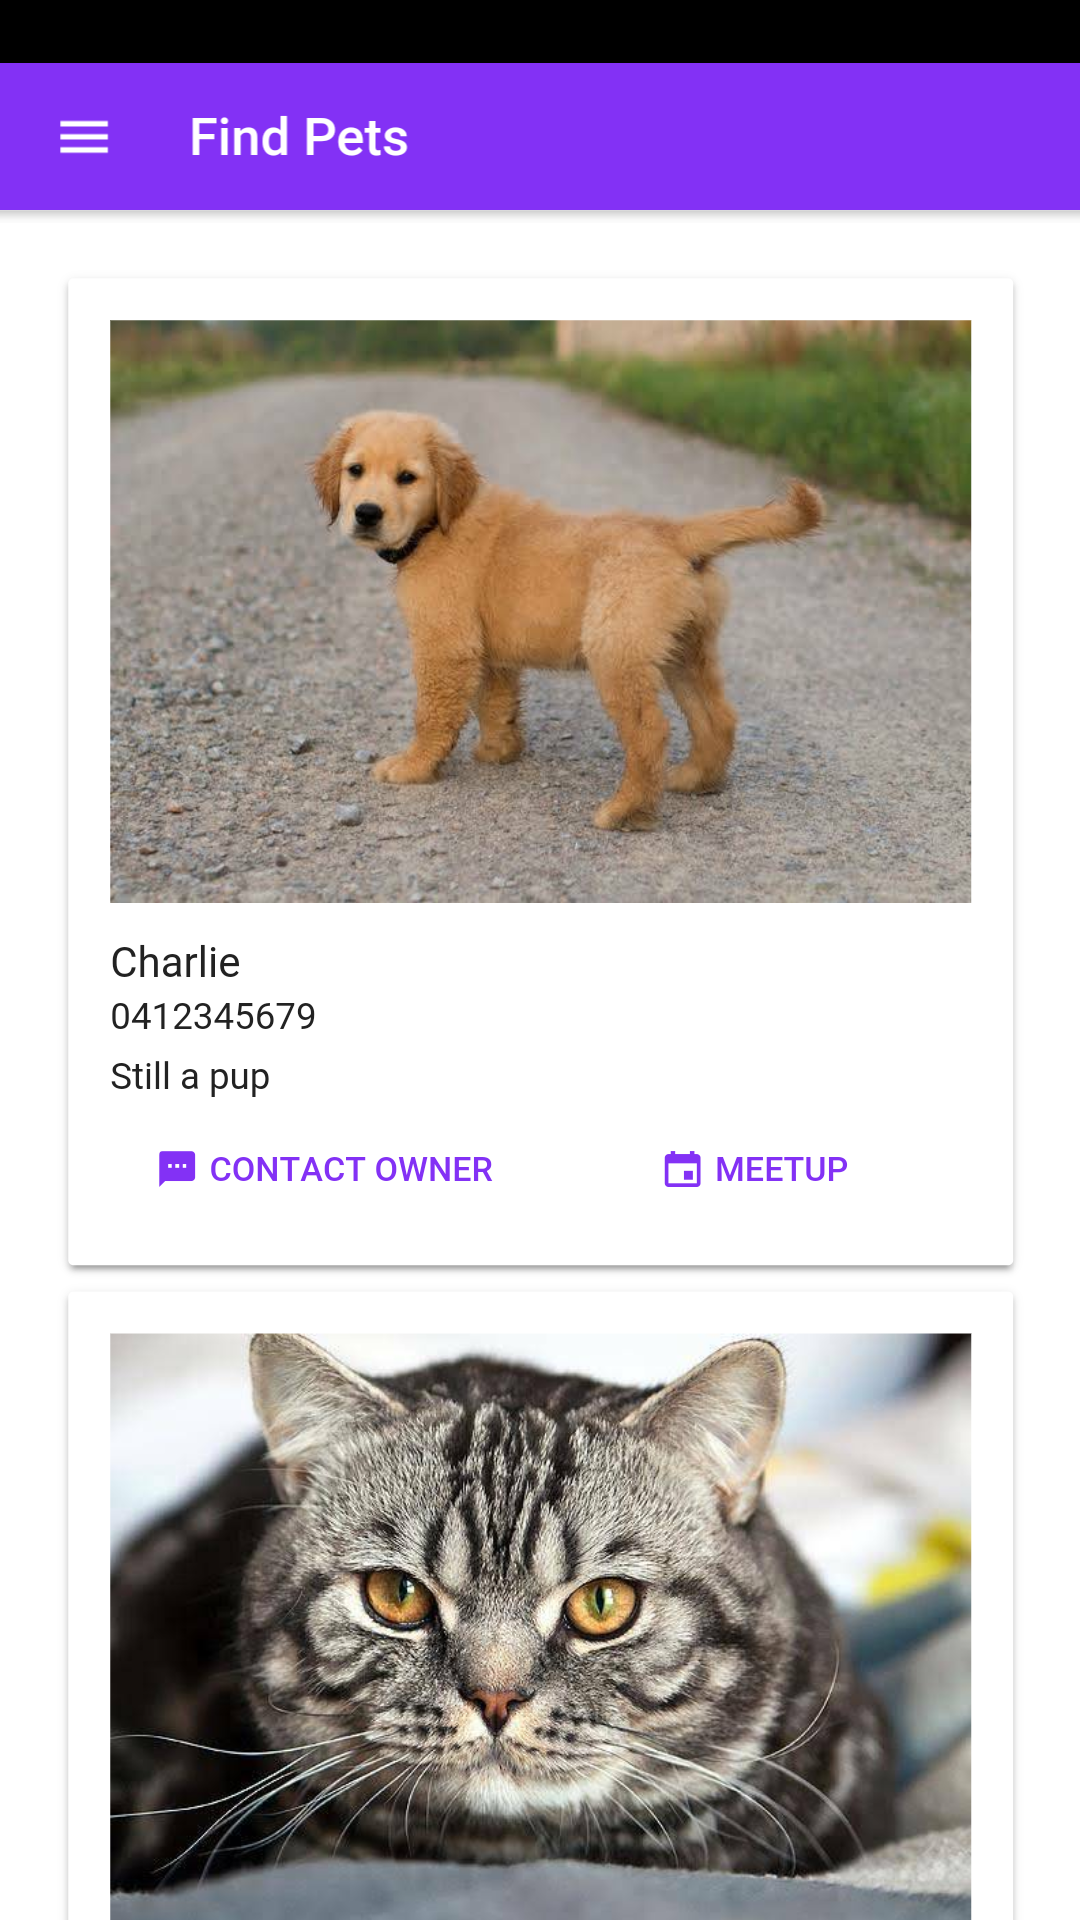
\includegraphics[scale=0.1]{find_pets.png} }}%
    \qquad
    \subfloat[A list of pets that a user owns]{{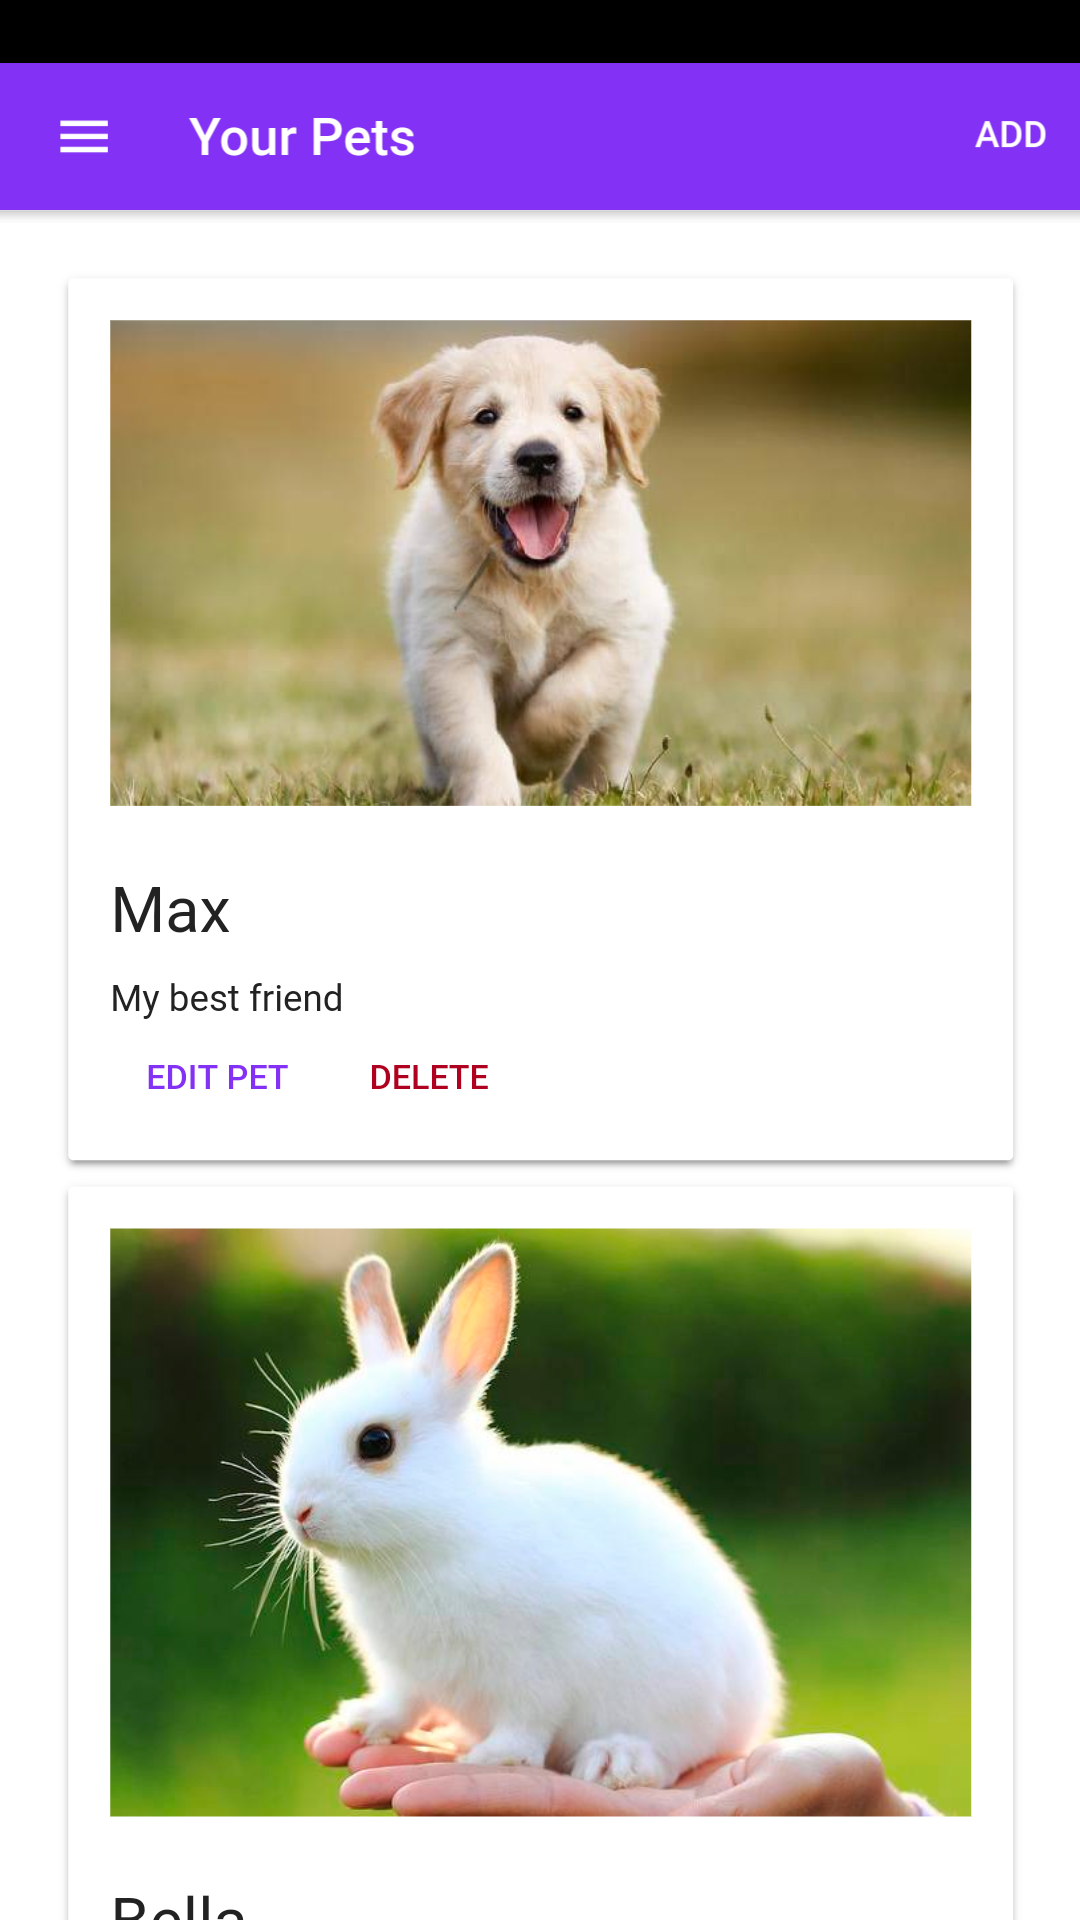
\includegraphics[scale=0.1]{your_pets.png} }}%
    \caption{Meetup For Pets Ionic 3 Application}%
    \label{fig:meetupIonic}%
\end{figure}
\\ In a real-world scenario, an application would normally take advantage of the hardware capabilities of the device it is running on. 
Therefore, there are some Ionic native framework features that were included, such as camera, contacts, calendar, and messaging.
\\ Using the case study above, we attempted to perform some manual migration to look deeper into the issues that may arise when migrating. 

\subsection{The Modelling Tool}
\section{Evaluation}

The results of the migration tool we developed were quite favorable. The case study
involved migrating three categories of changes:
\begin{enumerate}
    \item HTML markup
    \item Typescript code
    \item Architectural changes (file and folder structure)
\end{enumerate}

\subsection{HTML Markup}
The migration tool tackles the problem by separating the full
text into components (.i.e buttons, labels, etc.). This is the most
general category, as the migration process for different components
has a lot of common procedures.

\begin{figure}
    \centering
    \subfloat[Ionic 3]{
        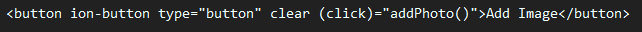
\includegraphics[width=0.8\linewidth]{button.PNG}
        \label{fig:ion3button}
    }
    \qquad
    \subfloat[Ionic 4]{
        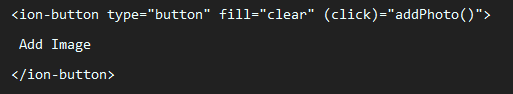
\includegraphics[width=0.8\linewidth]{buttonv4.PNG}
        \label{fig:ion4button}
    }
    \caption{Ionic 3-4 Button Migration (Markup)}
    \label{fig:ionicButtonMigration}
\end{figure}

\subsection{Typescript code}
Migration of Typescript code involves looking through code files
to find specific tokens and changing them to fit the Ionic 4 specification.
Unlike HTML markup, every different migration process in this category is almost
completely different, and can only be generalized in broad terms, such as find-and-replace
functionality.

\begin{figure}
    \centering
    \subfloat[Ionic 3]{
        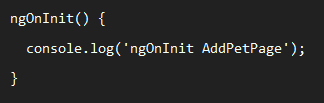
\includegraphics[width=0.8\linewidth]{lifecycle.PNG}
        \label{fig:lifecycle3}
    }
    \qquad
    \subfloat[Ionic 4]{
        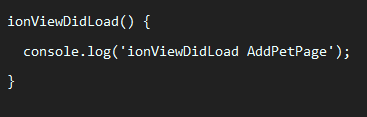
\includegraphics[width=0.8\linewidth]{lifecyclev4.PNG}
        \label{fig:lifecycle4}
    }
    \caption{Ionic 3-4 Lifecycle Methods Migration (Typescript)}
    \label{fig:ionicLifecycleMigration}
\end{figure}

\subsection{Architectural Changes}
The structure of an Ionic 4 project is drastically different from an Ionic 3 project,
making its migration a very specific process. The tool focuses on a small subset, which
involves reorganizing files associated with one specific feature of an app to the equivalent Ionic 4
folder structure, as well as renaming them to fit the new convention.

\begin{figure}
    \centering
    \subfloat[Ionic Feature Migration Output]{
        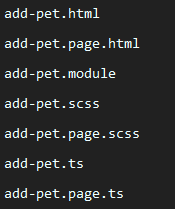
\includegraphics[width=0.8\linewidth]{files.PNG}
        \label{fig:ionFiles}
    }
    \caption{Ionic 3-4 File Rename-and-Relocate Migration (Architectural)}
    \label{fig:ionicFileMigration}
\end{figure}


\section{Discussion/Experiences}
The overall consensus is that model-driven development is a feasible approach
for software migration, especially regarding this case study in particular.
\newline \newline
For HTML markup in particular, automating component-wise migration is remarkably simple, and it
is well within the scope of possibility to create a general function that will migrate any Ionic
3 component to its Ionic 4 equivalent, provided a library of changes specific to each component
is collated for use by this function.
\newline \newline
Typescript code can be a little more complicated to deal with. During development of the tool,
we encountered some difficulty with porting over two components in particular - \textbf{Toasts} and
\textbf{Alerts}. The difficulty stems from the asynchronous nature of the two in Ionic 4 as opposed to their
counterparts in Ionic 3 - handler function callbacks and deeply nested toasts and alerts have to be handled differently,
which makes migrating these a more involved process than just pure automation.
\newline \newline
Architectural changes vary in difficulty. A project-wide relocation and renaming of files is well within the
scope of possibility, but changes to the routing mechanisms adopted in the different versions are drastic and
require significant changes to the codebase. Ionic 4 uses the routing functionality provided by the frontend framework
specified when creating a project using its command-line interface, meaning that a separate migration process would need
to be adopted for, say, React vs. Angular, for example. Ionic 3 used its own proprietary router on the other hand, which means
at least that part of the code is easier to deal with. While Ionic 4 adopted this change in order to be future-proof, this does
make a generalized migration tool for this specific feature a lot harder to implement.

% @Author: Riordan Dervin Alfredo, 2/11/2019 %
\section{Related Work}
In regards to the software migration that utilises model driven engineering methods,
there are already several studies that were conducted extensively before.
Those are; FASMM: 
Fast and Accessible Software Migration Method \cite{b3}, Reverse Engineering 
Strategies for Software Migration \cite{b4}, Model-Driven Engineering 
for Software Migration in a Large Industrial Context \cite{b5},  
Towards a Model-Driven Approach for Planning a 
Standard-Based Migration of Enterprise Applications to SOA  \cite{b6}, and
Migrating C/C++ Software to Mobile Platforms in the ADM Context \cite{b2}

Our study is closely related to the FASMM approach \cite{b3} as this research
provides extensive guides for software developers that have limited 
resources (time, budget, workforce etc.) to conduct software migration. 
\cite{b4} study provides specific methods to conduct reverse-engineering 
that is involved our process.

In \cite{b5} and \cite{b6} studies are proving the feasibility of model-driven engineering
in different domains and contexts from our studies. Those are the migration to a completely new framework, 
migration to a new architecture (legacy achitecture to service-oriented architecture), and migration
of different languages to specific mobile application framework. 
They also provided insights on how model-driven engineering processes are economically
profitable and are cost-effective. 

This \cite{b2} study is related to our work in terms of processing different kinds of 
programming languages and paradigms to generate mobile application code. It is also 
the main feasible example of a model-driven approach in the software migration of mobile applications,
which is in our case is the migration of the hybrid mobile application.

The related work is explained in detail as shown below. 

\subsection{ FASMM: Fast and Accessible Software Migration Method }
% TODO: Add explanation for this paper, if page limit permits it %
\textcolor{blue}{<draft>}

\subsection{ Model-Driven Engineering for Software Migration in a Large Industrial Context }
This paper describes the process of migrating a large-scale software application from Mainframe to J2EE
using Model-Driven Engineering process. The migration process in this study starts by describing the general 
processes of the current legacy system.

First, a parser is created to make an abstract systax tree from the legacy code. Then, it is processed
by a transformation to build a model that conforms to the meta-model of the legacy language.
During the second stage, all symbols are resolved and bound to the appropriate model elements.

Afterwards, from the model representing the code, a reverse-engineering process is conducted to produce a platform independent 
model. Finally, this model will be mapped into a platform specific model that can be used to generate code
for the final product of the migrated application. 

\subsection{ Towards a Model-Driven Approach for Planning a Standard-Based Migration of Enterprise Applications to SOA }
% TODO: Add explanation for this paper, if page limit permits it %
\textcolor{blue}{<draft>}

\subsection{ Migrating C/C++ Software to Mobile Platforms in the ADM Context }
This study took an example of C/C++ language to produce an Android, iOS, and Windows mobile application. 
In our study, the extension type of the generated code is still maintained,
but the main code-generation process is technically similar. 

Furthermore, this study gives insight in regards to the feasibility of a model-driven development approach that is 
advanced to ADM (Architecture-Driven Modernization) within a similar domain, mobile application migration. 
The ADM approach that is described in this study could potentially be part of our future works. 
The validation tool that is used in this study is the same as what we are using in our approach, which is the Eclipse Modelling Framework.
Mobile applications are formed using different kinds of programming languages, which is technically 
how hybrid application systems work. 

\section{Conclusion}
In conclusion, our study contributes to the success and feasibility for another area 
of software migration with model-driven engineering methodologies, focusing on the hybrid application domain.
At this stage, our approach only proves a small fraction of the hybrid application domain because 
this study only focused on one framework (Ionic) and selected specific versions (migrating version 3 to version 4). 

At the moment, within these constraints, the tool that we had created only handles basic migration functionalities.
More specifically it is only using string parsing, transformations, and code-generation. These processes might
be insufficient to handle more complex functionalities as described in our limitations.

There are still many other challenges to tackle in the proposed methods to fully migrate the Ionic version 3 project
to version 4. This is due to our proposed approach focusing on the feasibility of the concept of attempting to migrate the hybrid application 
completely. Despite all of these challenges and limitations, our approach could potentitally open-up more paths for further research
in the software migration of hybrid applications by utilising model-driven engineering approaches.  

\section{Future Work}
Here, we used the Eclipse Modeling Framework as our validator and main tool to help migrate the Ionic framework 
from version 3 to version 4. Within this tool, the abstraction level is intentionally increased for the 
cohesiveness and extensibility of migration functions. while also reducing coupling between 
functions. Future researchers could upgrade more complex functionalities based on the limitations that 
we had listed above.

The main reason is the tool that we had created was only able to solve basic migration problems. 
It requires more extensive research to solve more complex functionalites, such as dealing with 
architectural changes to arrange files in the correct directories. The potential of
higher-level model-driven approaches could possibly be exercised in ADM (Architecture-Driven Modernization) \cite{b2}. 

There will be time in the future for this tool to be mature so that it can migrate Ionic Framework applications from version 
3 to version 4 thoroughly, without introducing any migration bugs.
This tool is also envisioned to handle migration of Ionic framework from 
any versions to the latest. In the future, by following our approaches and adding on further research, 
it could potentially migrate other different hybrid application framework versions as well.

\begin{thebibliography}{00}
\bibitem{b1} "IBM Knowledge Center", Ibm.com, 2019. [Online]. Available: \url{https://www.ibm.com/support/knowledgecenter/en/SSEP7J_10.2.1/com.ibm.swg.ba.cognos.ug_mfdm.10.2.1.doc/c_mfdm_chal_mig.html}. [Accessed: 07-Sep-2019].
% Related works' biblioraphies %
\bibitem{b2} Martinez, L., et al. ``Migrating C/C++ Software to Mobile Platforms in the ADM context,'' \textit{International Journal of Interactive Multimedia and Artificial Intelligence}, Vol. 4 , N\textsuperscript{o}3, p. 34, 2017. [Abstract]. Available: Semantics Scholar, URL: \url{https://pdfs.semanticscholar.org/8968/7958518252817c4bbe02c77fcef5a48a8d3c.pdf}, [Accessed November 1, 2019].
\bibitem{b3} Forite, L. and C. Hug. ``FASMM: Fast and Accessible Software Migration Method,'' in Research Challenges in Information Science (RCIS), 2014 IEEE Eights Internation Conference on. 2014, IEEE.
\bibitem{b4} Muller, H. A. ``Reverse Engineering Strategies for Software Migration'', in Proceedings of the (19\textsuperscript{th}) International Conference on Software Engineering, May 1997, p. 659, IEEE.
\bibitem{b5} Fleurey, F., et al. ``Model-Driven Engineering for Software Migration in a Large Industrial Context'', in International Conference on Model Driven Engineering Languages and Systems, 2007, pp. 482-497, MODELS
\bibitem{b6} Aboulsamh, M.A. ``Towards a Model-Driven Approach for Planning a Standard-Based Migration of Enterprise Applications to SOA'', in 2009 Congress on Services - l , 2009, IEEE.

\end{thebibliography}
\vspace{12pt}
\color{red}

\end{document}
